\documentclass{beamer}

%\usetheme{Singapore}
%\usetheme{Hannover}
%\usetheme{Szeged}
\usetheme{Montpellier}
\usecolortheme{dove}
%\usecolortheme{lily}
%\usecolortheme{rose}

\useinnertheme[shadow]{rounded} 


\newtheorem{remark}{Remark}

\usepackage{listings}
\usepackage{haskell,proof}
\usepackage{fancyvrb,alltt}
\usepackage{amsmath}
%\usepackage{beamerthemesplit}
\renewcommand{\ttdefault}{pcr}
\definecolor{gray_ulisses}{gray}{0.55}
\definecolor{castanho_ulisses}{rgb}{0.71,0.33,0.14}
\definecolor{preto_ulisses}{rgb}{0.41,0.20,0.04}
\definecolor{green_ulises}{rgb}{0.2,0.75,0}
\lstdefinelanguage{HaskellUlisses} {
        basicstyle=\itfamily\small,
        sensitive=true,
        morecomment=[l][\ttfamily\tiny]{--},
        morecomment=[s][\ttfamily\tiny]{\{-}{-\}},
%       morecomment=[l][\color{gray_ulisses}\ttfamily]{--},
%       morecomment=[s][\color{gray_ulisses}\ttfamily]{\{-}{-\}},
%       morecomment=[l][\color{gray_ulisses}\ttfamily\tiny]{--},
%       morecomment=[s][\color{gray_ulisses}\ttfamily\tiny]{\{-}{-\}},
        morestring=[b]",
        %stringstyle=\color{red},
        showstringspaces=false,
        numberstyle=\tiny,
        numberblanklines=true,
        showspaces=false,
        breaklines=true,
        showtabs=false,
        emph=
        {[1]
                        FilePath,IOError,abs,acos,acosh,all,and,any,appendFile,approxRational,asTypeOf,asin,
                asinh,atan,atan2,atanh,basicIORun,break,catch,ceiling,chr,compare,concat,concatMap,
                const,cos,cosh,curry,cycle,decodeFloat,denominator,digitToInt,div,divMod,drop,
                dropWhile,either,elem,encodeFloat,enumFrom,enumFromThen,enumFromThenTo,enumFromTo,
                error,even,exponent,fail,filter,flip,floatDigits,floatRadix,floatRange,floor,
                fmap,foldl,foldl1,foldr,foldr1,fromDouble,fromEnum,fromInt,fromInteger,fromIntegral,
                fromRational,gcd,getChar,getContents,getLine,head,id,inRange,index,init,intToDigit,
                interact,ioError,isAlpha,isAlphaNum,isAscii,isControl,isDenormalized,isDigit,isHexDigit,
                isIEEE,isInfinite,isLower,isNaN,isNegativeZero,isOctDigit,isPrint,isSpace,isUpper,iterate,iter,iterS,
                last,lcm,length,lex,lexDigits,lexLitChar,lines,log,logBase,lookup,map,mapM,mapM_,max,
                maxBound,maximum,maybe,min,minBound,minimum,mod,negate,not,notElem,null,numerator,odd,
                or,ord,pi,pred,primExitWith,print,product,properFraction,putChar,putStr,putStrLn,quot,
                quotRem,range,rangeSize,read,readDec,readFile,readFloat,readHex,readIO,readInt,readList,readLitChar,
                readLn,readOct,readParen,readSigned,reads,readsPrec,realToFrac,recip,refold,rem,replicate,
                reverse,round,scaleFloat,scanl,scanl1,scanr,scanr1,seq,sequence,sequence_,show,showChar,showInt,
                showList,showLitChar,showParen,showSigned,showString,shows,showsPrec,significand,signum,sin,
                sinh,snd,span,splitAt,sqrt,subtract,succ,sum,tail,take,takeWhile,tan,tanh,threadToIOResult,toEnum,
                toInt,toInteger,toLower,toRational,toUpper,truncate,uncurry,unlines,until,unwords,unzip,
                unzip3,userError,words,writeFile,zip,zip3,zipWith,zipWith3,listArray,doParse,lift,signal,get,put,extrude,return
        },
        emphstyle={[1]\textbf},
        emph=
        {[2]
                Double,Either,IO,Ordering,Rational,Ratio,ReadS,ShowS,
                Word8,InPacket,ReT,StT,I
        },
        emphstyle={[2]\textbf},
        emph=
        {[3]
                case,class,deriving,do,else,if,import,in,infixl,infixr,instance,let,
                module,of,primitive,then,data,type,vhdl,newtype
        },
        emphstyle={[3]\textbf},
        emph=
        {[4]
                quot,rem,div,mod,elem,notElem,seq
        },
%        emphstyle={[4]\color{castanho_ulisses}\textbf},
        emphstyle={[4]\textbf},
        emph=
        {[5]
                False,Just,Left,Nothing,Right,Show,Eq,Ord,Num
        },
%        emphstyle={[5]\color{preto_ulisses}\textbf}
        emphstyle={[5]\textbf}
}

\lstnewenvironment{footcode}
}
{}
%{\hrulesmallskip} not sure what this is.

%\lstnewenvironment{hcode}
%{%\textbf{Haskell Code} \hspace{1cm} \hrulefill
% \lstset{language=HaskellUlisses,    basicstyle=\ttfamily\small,escapechar=\%}}
%{}

\lstnewenvironment{hcode}
}
{}

\lstnewenvironment{smallcode}
{%\hspace{1cm}
 \lstset{language=HaskellUlisses,       basicstyle=\ttfamily\small,escapechar=\%
}}
{}
%{\hrulesmallskip} not sure what this is.

\lstnewenvironment{tinycode}
{%\hspace{1cm}
 \lstset{language=HaskellUlisses,       basicstyle=\ttfamily\scriptsize,escapechar=\%
}}
{}

\lstnewenvironment{teenycode}
{%\hspace{1cm}
 \lstset{language=HaskellUlisses,       basicstyle=\ttfamily\tiny,escapechar=\%
}}
{}


\lstnewenvironment{newcode}{\lstset{language=Haskell,basicstyle=\scriptsize,identifierstyle=\itshape,stringstyle=\itshape,escapechar=\%}}{}

\lstnewenvironment{normalcode}{\lstset{language=Haskell,
                                       basicstyle=\normalsize\ttfamily,
                                       keywordstyle=\bfseries,
                                       %identifierstyle=\itshape,
                                       %stringstyle=\itshape,
                                       escapechar=\%}}{}

\lstnewenvironment{vhdl}
{\lstset{language=VHDL,basicstyle=\ttfamily\small,escapechar=\%}}{}

\lstdefinelanguage{PreHDL} {
        basicstyle=\ttfamily\small,
        sensitive=true,
        morecomment=[l][\ttfamily\tiny]{//},
%        morecomment=[s][\ttfamily\tiny]{\{-}{-\}},
%       morecomment=[l][\color{gray_ulisses}\ttfamily]{--},
%       morecomment=[s][\color{gray_ulisses}\ttfamily]{\{-}{-\}},
%       morecomment=[l][\color{gray_ulisses}\ttfamily\tiny]{--},
%       morecomment=[s][\color{gray_ulisses}\ttfamily\tiny]{\{-}{-\}},
        morestring=[b]",
        %stringstyle=\color{red},
        showstringspaces=false,
        numberstyle=\tiny,
        numberblanklines=true,
        showspaces=false,
        breaklines=true,
        showtabs=false,
        emph=
        {[1]
                input,output,vhdl,label,if,else,yield,goto,boolean,bits,true,false,function,return,concat
        },
        emphstyle={[1]\textbf}
}

\lstnewenvironment{prehdl}
{\lstset{language=PreHDL,basicstyle=\ttfamily\small,escapechar=\%}}{}

\newcommand{\ra}{\ensuremath{\rightarrow}}
\newcommand{\edit}[1]{\marginpar{\raggedright\tiny\it{#1}}}

\newcommand{\incode}[1]{{\footnotesize{\tt{#1}}}}


\newcommand{\modal}[2]{\ensuremath{\mathsf{#1}_{#2}}}
\newcommand{\kripke}[1]{\ensuremath{\sim_{#1}}}
\renewcommand{\implies}{\ensuremath{\supset}}
\newcommand{\hbind}[1]{\ensuremath{\mbox{{\footnotesize{\texttt{{>}{>}{=}}}}}_{\mbox{\tiny {\it #1}}}}}
\newcommand{\hbindnull}[1]{\ensuremath{\footnotesize{\texttt{{>}{>}}}_{\mbox{\tiny {\it #1}}}}}
\newcommand{\hreturn}[1]{\ensuremath{\mathtt{return}_{\mbox{\tiny {\it #1}}}}}
%\renewcommand{\code}[1]{\ensuremath{\mathtt{#1}}}
\newcommand{\tyjudgment}[3]{\ensuremath{#1 \triangleright #2 : #3 }}
\newcommand{\nil}{\ensuremath{\mathtt{()}}}
\newcommand{\hmodels}{\tiny{\ddtstile{}{}}}
\newcommand*\widebar[1]{%
  \hbox{%
    \vbox{%
      \hrule height 0.5pt % The actual bar
      \kern0.1ex%         % Distance between bar and symbol
      \hbox{%
        \kern-0.1em%      % Shortening on the left side
        \ensuremath{#1}%
        \kern-0.1em%      % Shortening on the right side
      }%
    }%
  }%
} 

\newcommand{\parS}{\ensuremath{{{.}{\mathtt{\&}}{.}}}}
\newcommand{\parA}{\ensuremath{{{.}{\ast}{.}}}}
%\newcommand{\pardev}{\ensuremath{{{\mathtt{<}}{\mathtt{\&}}{\mathtt{>}}}}}
\newcommand{\pardev}{\ensuremath{\mbox{{\texttt{<\&>}}}}}



%\newcommand{\tyjudgment}[3]{\ensuremath{#1 \triangleright #2 : #3 }}
\newcommand{\judgment}[3]{\ensuremath{#1 \vdash #2 : #3}}
%\lstnewenvironment{newcode}{\lstset{language=Haskell,basicstyle=\scriptsize,escapechar=\@}}{}
\newcommand{\ttcode}[1]{{\color{red}{\tt{#1}}}}
\newcommand{\lang}[1]{\ensuremath{\mathcal{L}(#1)}}

\newcommand{\forget}[1]{}
\title{A Type-based Approach to Program Security}
\subtitle{Dennis Volpano \& Geoffrey Smith, TAPSOFT 1997}
\author{Professor William L. Harrison\\CS8440 Fall 2015}
\date{\today}

\begin{document}


\frame{\titlepage}

%%%%%%%%%%%%%%%%%%%%%%%%%%
%%%%%%%%%%%%%%%%%%%%%%%%%%
%%%%%%%%%%%%%%%%%%%%%%%%%%
%%%%%%%%%%%%%%%%%%%%%%%%%%
%%%%%%%%%%%%%%%%%%%%%%%%%%
\begin{frame}[fragile]
\frametitle{Overview}


\begin{itemize}
\item Retrofits noninterference to programming languages
\pause
\item Ex: Consider the following procedure: 
\begin{haskell}
proc P(inout x : low, inout y : high)
\end{haskell}
\pause
\item Suppose \<P(u:low, v:high)\> and \<P(u:low,w:high)\> terminate
      with values \<u\>, \<v\> and \<w\>.
\pause
\item The final values for \<v\> and \<w\> may differ, 
 {\bf but}, if \<P\> is noninterfering, then the final values for \<u\> must be identical.
\pause
\item Smith \& Volpano's type system enforces noninterference---\<P\> is well-typed means it's noninterfering.
\end{itemize}

\end{frame}

%%%%%%%%%%%%%%%%%%%%%%%%%%%%%%%%%%%%%%%%%%%%%%
%%%%%%%%%%%%%%%%%%%%%%%%%%%%%%%%%%%%%%%%%%%%%%
%%%%%%%%%%%%%%%%%%%%%%%%%%%%%%%%%%%%%%%%%%%%%%
%%%%%%%%%%%%%%%%%%%%%%%%%%%%%%%%%%%%%%%%%%%%%%
%%%%%%%%%%%%%%%%%%%%%%%%%%%%%%%%%%%%%%%%%%%%%%
\section{Typing Information Flows}

\begin{frame}[fragile]
\frametitle{Explicit Flows}

\begin{itemize}
\item For \<l : low var\> and \<h : high var\>,
      an explicit flow \<l := h\> must be rejected.
\pause
\item In Denning \& Denning, this was performed by the certification mechanism.
\pause
\item In Smith and Volpano, this is accomplished via a typing rule:
\begin{haskell}
\infer[]{\gamma \vdash e := e' : \tau cmd}{\gamma \vdash e : \tau acc & \gamma \vdash e' : \tau}
\end{haskell} 
\pause 
\item This rule insists that \<h\> and \<l\> be typed on the same level. How?
\end{itemize}

\end{frame}
%%%%%%%%%%%%%%%%%%%%%%%%%%
%%%%%%%%%%%%%%%%%%%%%%%%%%
%%%%%%%%%%%%%%%%%%%%%%%%%%
%%%%%%%%%%%%%%%%%%%%%%%%%%
%%%%%%%%%%%%%%%%%%%%%%%%%%
\begin{frame}[fragile]
\frametitle{Running Example}

\begin{center}
\begin{normalcode}
            while h > 0 do
               l := l + 1;
               h := h - 1
            od 
\end{normalcode}
\end{center}
\pause
\begin{itemize}
\item Q: What kind of flows exist in this program?
\end{itemize}

\end{frame}

\begin{frame}[fragile]
\frametitle{Running Example}

\begin{center}
\begin{normalcode}
            while h > 0 do
               l := l + 1;
               h := h - 1
            od 
\end{normalcode}
\end{center}
\pause
\begin{itemize}
\item The typing rule for \<while\> insists that the test and body of the loop be typed at the same level:
\begin{haskell}
\infer[]{\gamma \vdash while e do c : \tau cmd}{\gamma \vdash e : \tau & \gamma \vdash c : \tau cmd}
\end{haskell}
\end{itemize}

\end{frame}

\section{Introduction to the Type System}

\begin{frame}[fragile]
\frametitle{Programming Language Syntax}

\begin{center}
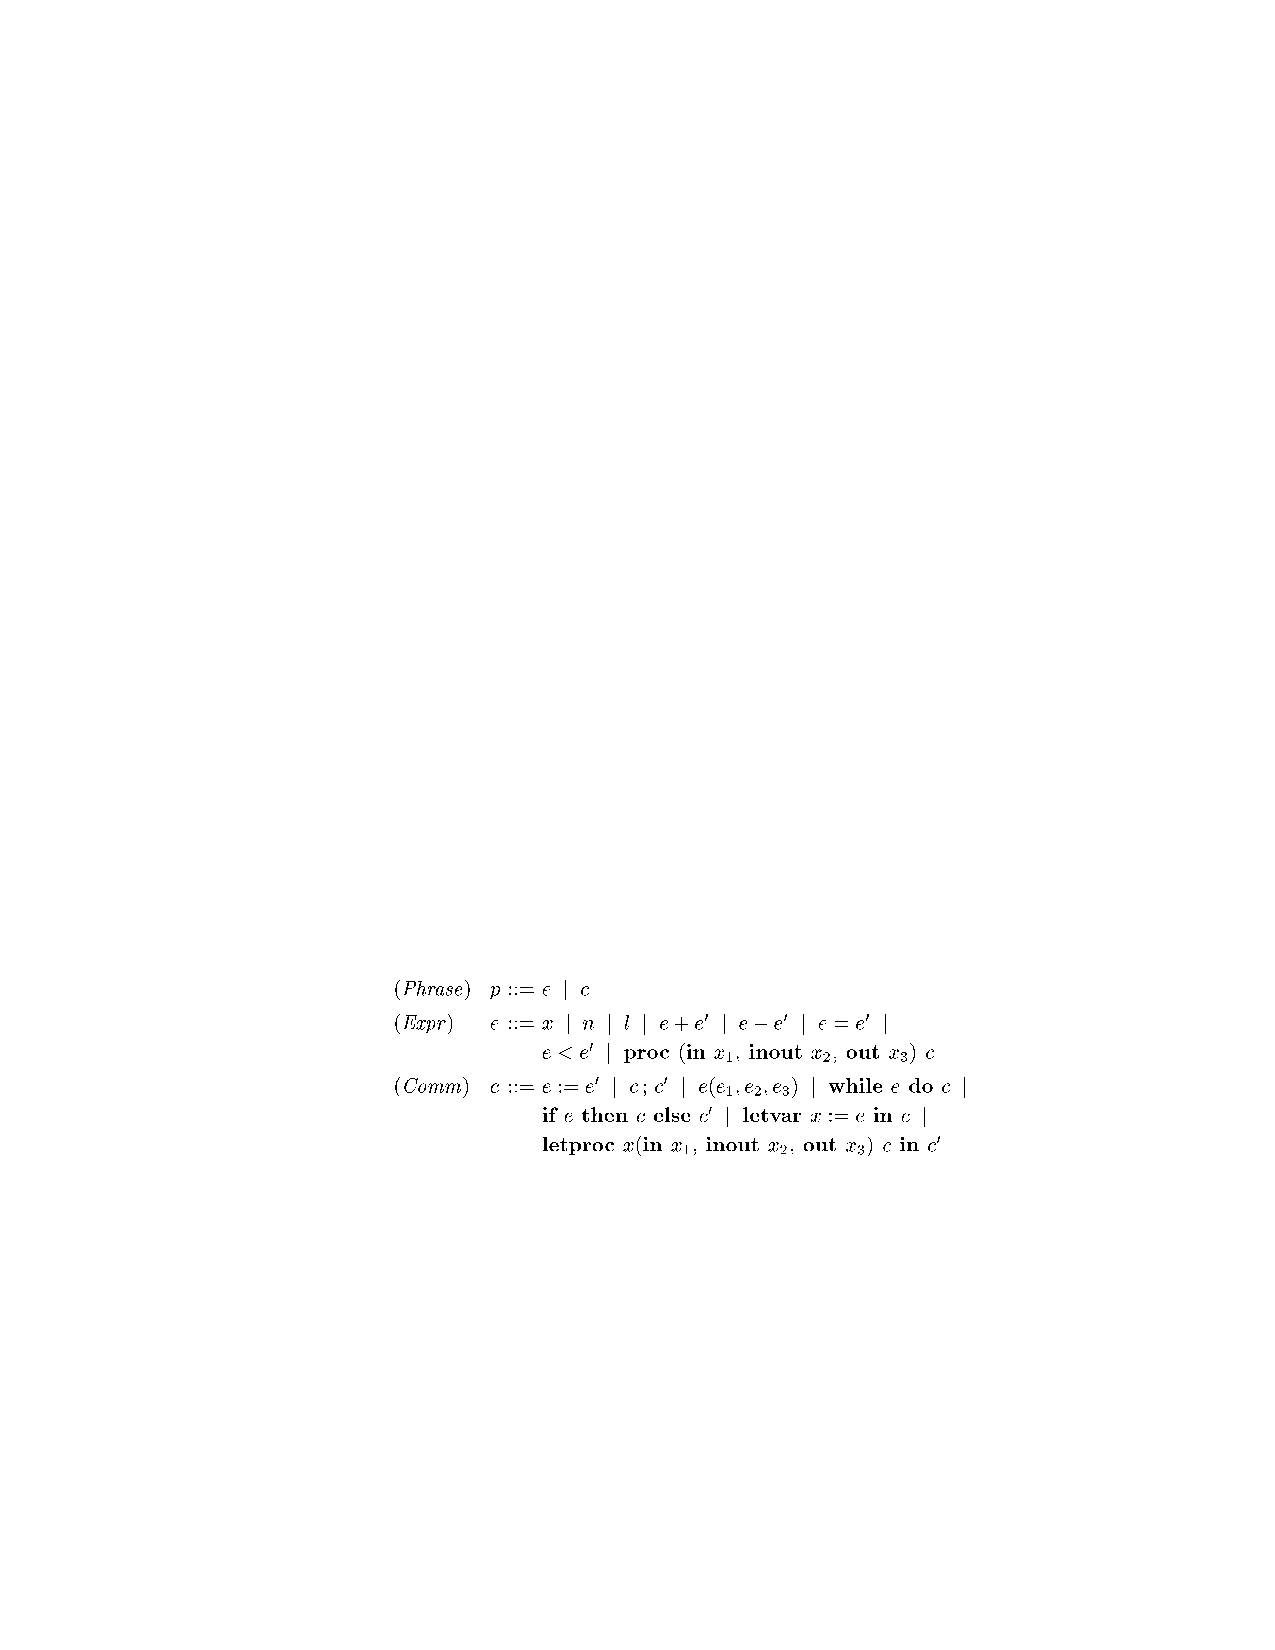
\includegraphics[scale=1.0]{figures/languagesyntax}
\end{center}

\end{frame}

\begin{frame}[fragile]
\frametitle{Type Syntax}

\begin{center}
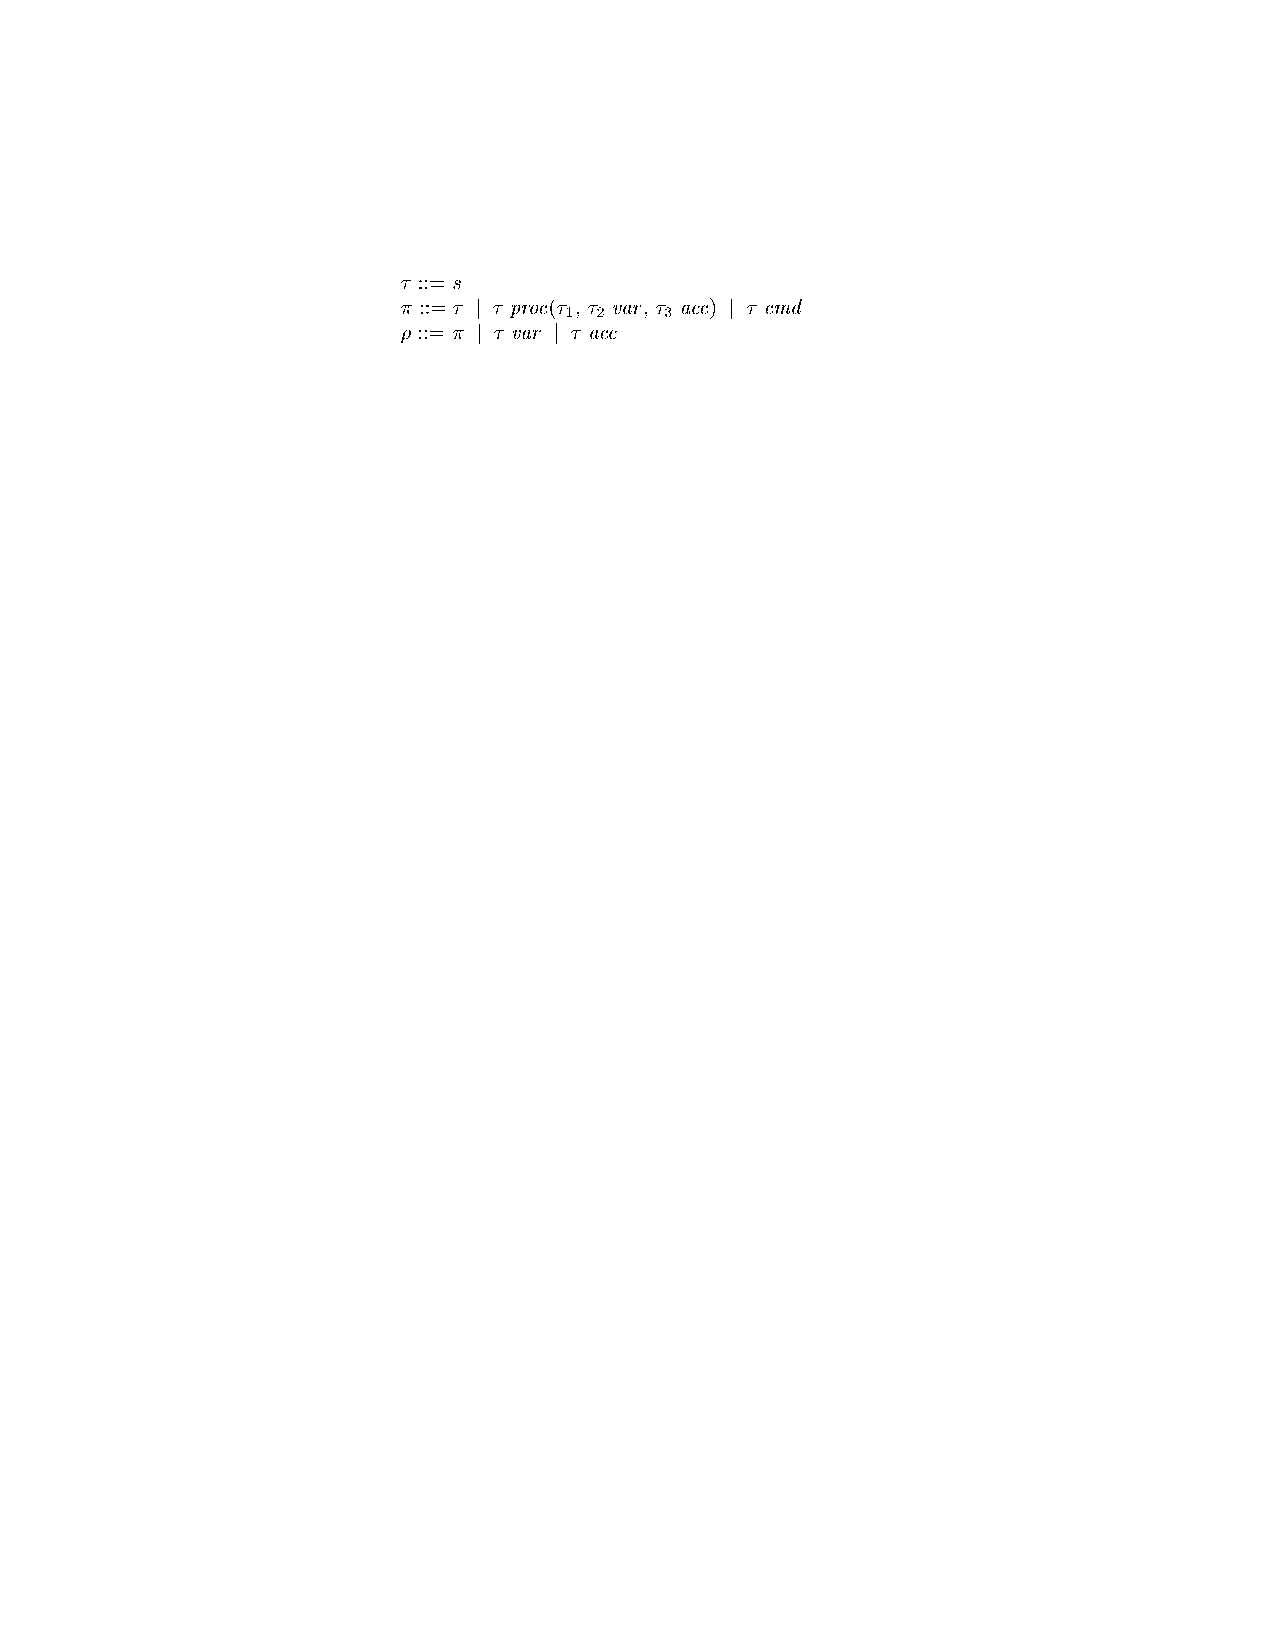
\includegraphics[scale=1.5]{figures/typesyntax}
\end{center}

N.b., $s$ is a \emph{security level}. It is assumed that all security levels form a lattice ordered by $\leq$.

\end{frame}

\begin{frame}[fragile]
\frametitle{Type Judgments}
{\Large
\[
\judgment{\lambda ; \gamma}{e}{\rho}
\]
}

\pause
\begin{itemize}
\item $e$ is a program phrase (i.e., expression, command, etc.).
\pause
\item $\rho$ is a type.
\pause
\item $\gamma$ is the \emph{identifier typing environment}.\\~~~~N.b., ``$\gamma(i) = \rho$'' means $i$ has type $\rho$ in $\gamma$.
\pause
\item $\lambda$ is the \emph{location typing environment}.
\begin{itemize}
\item Locations are used for input-output in the semantics.
\item Locations are, in effect, global.
\item $\lambda$ largely irrelevant to the type system; only occurs in one rule (VARLOC).
\end{itemize}
\end{itemize}

\end{frame}

%%%%%%%%%%%%%%%%%%%%%%%%%%
%%%%%%%%%%%%%%%%%%%%%%%%%%
%%%%%%%%%%%%%%%%%%%%%%%%%%
%%%%%%%%%%%%%%%%%%%%%%%%%%
%%%%%%%%%%%%%%%%%%%%%%%%%%

\section{Formal Treatment of Type System}


\begin{frame}[fragile]
\begin{center}
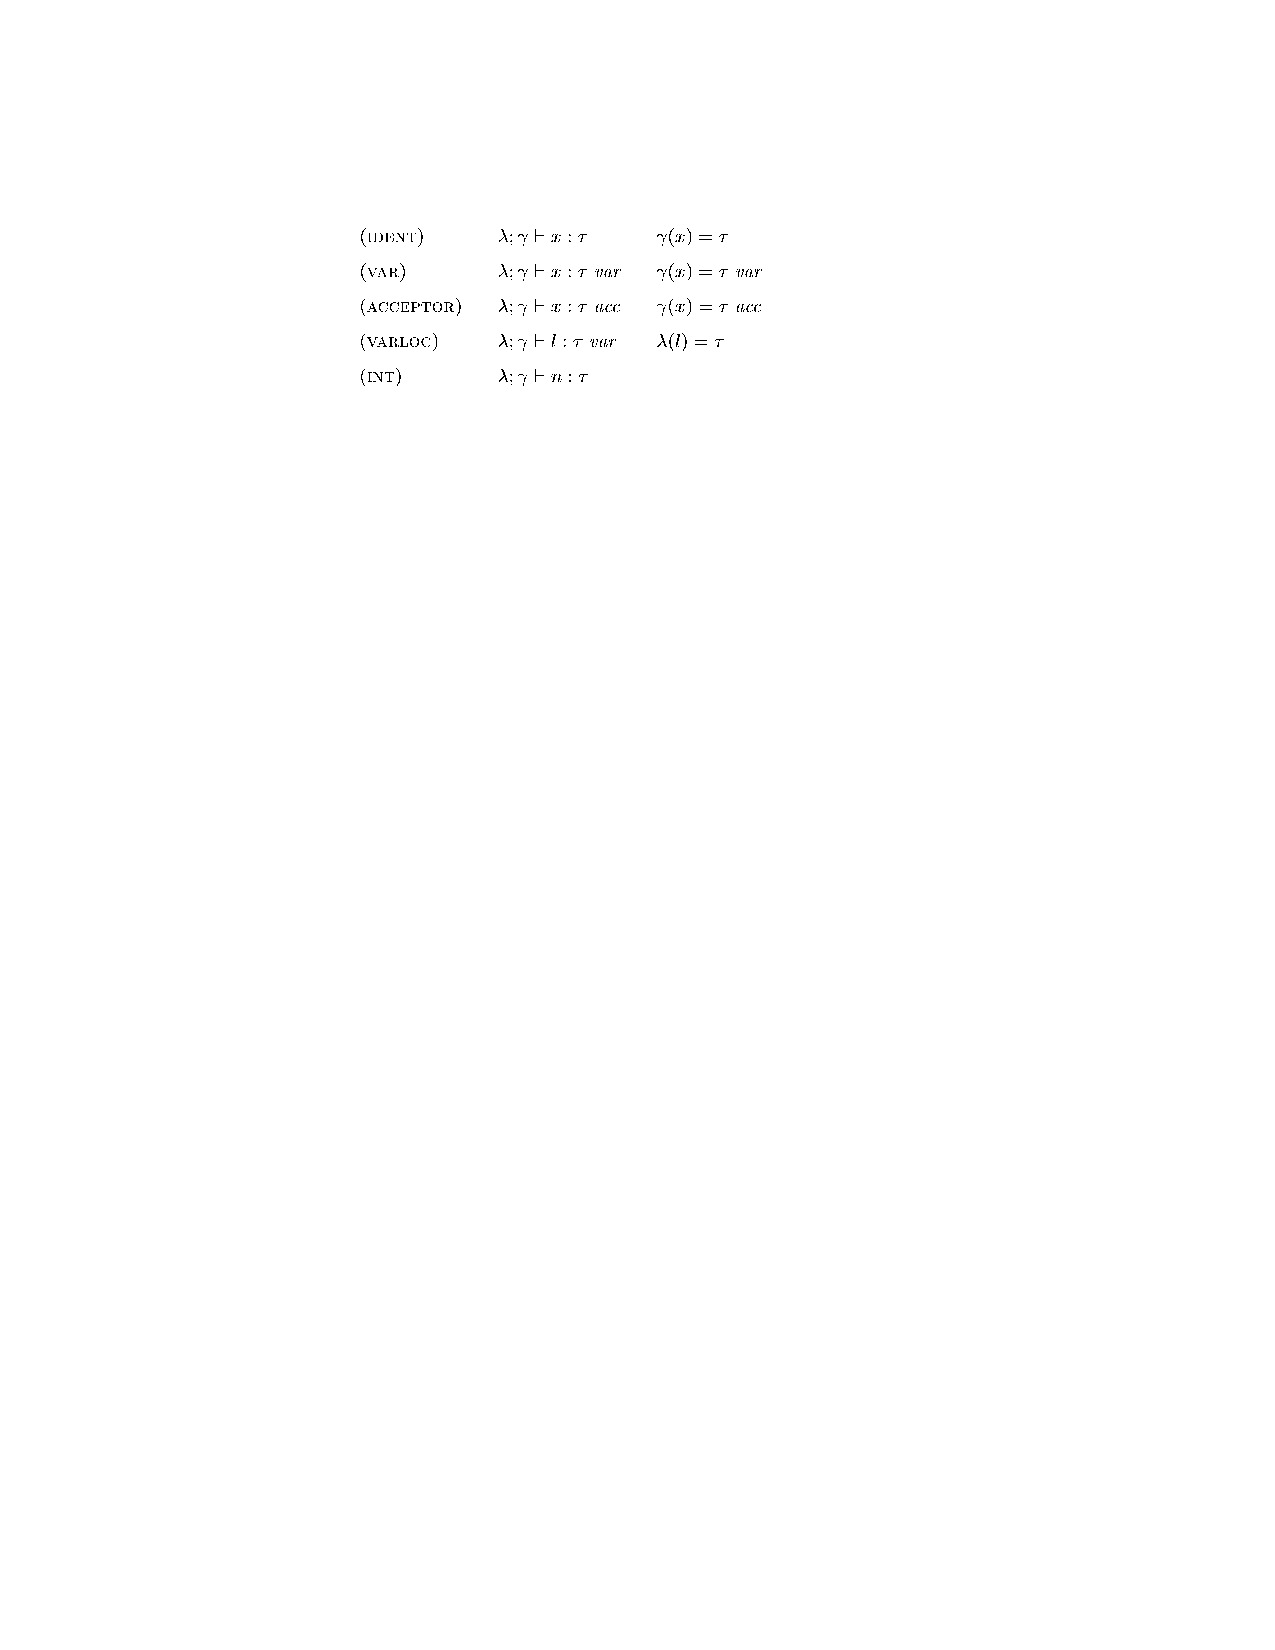
\includegraphics[scale=1.2]{figures/typesys1}
\end{center}
\end{frame}

    
\begin{frame}[fragile]
\begin{center}
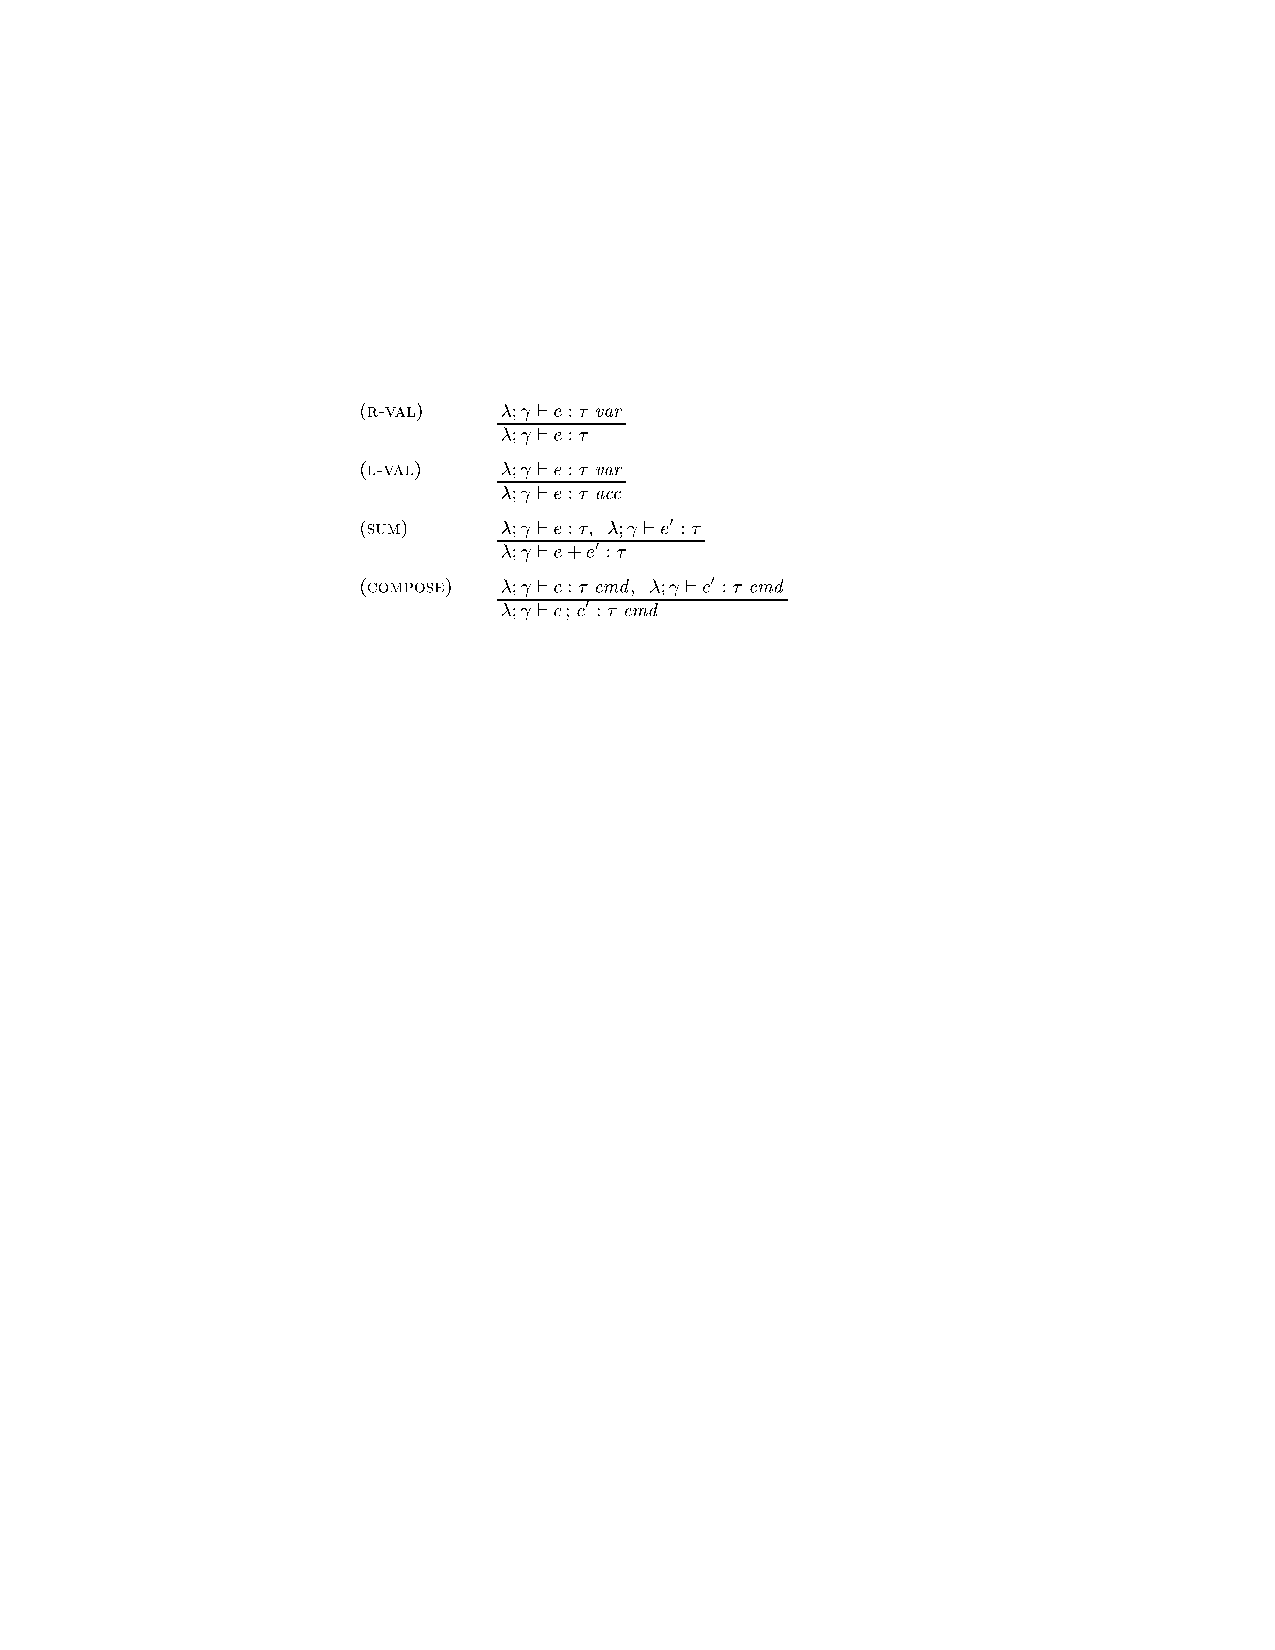
\includegraphics[scale=1.2]{figures/typesys2}
\end{center}
\end{frame}
    
\begin{frame}[fragile]
\begin{center}
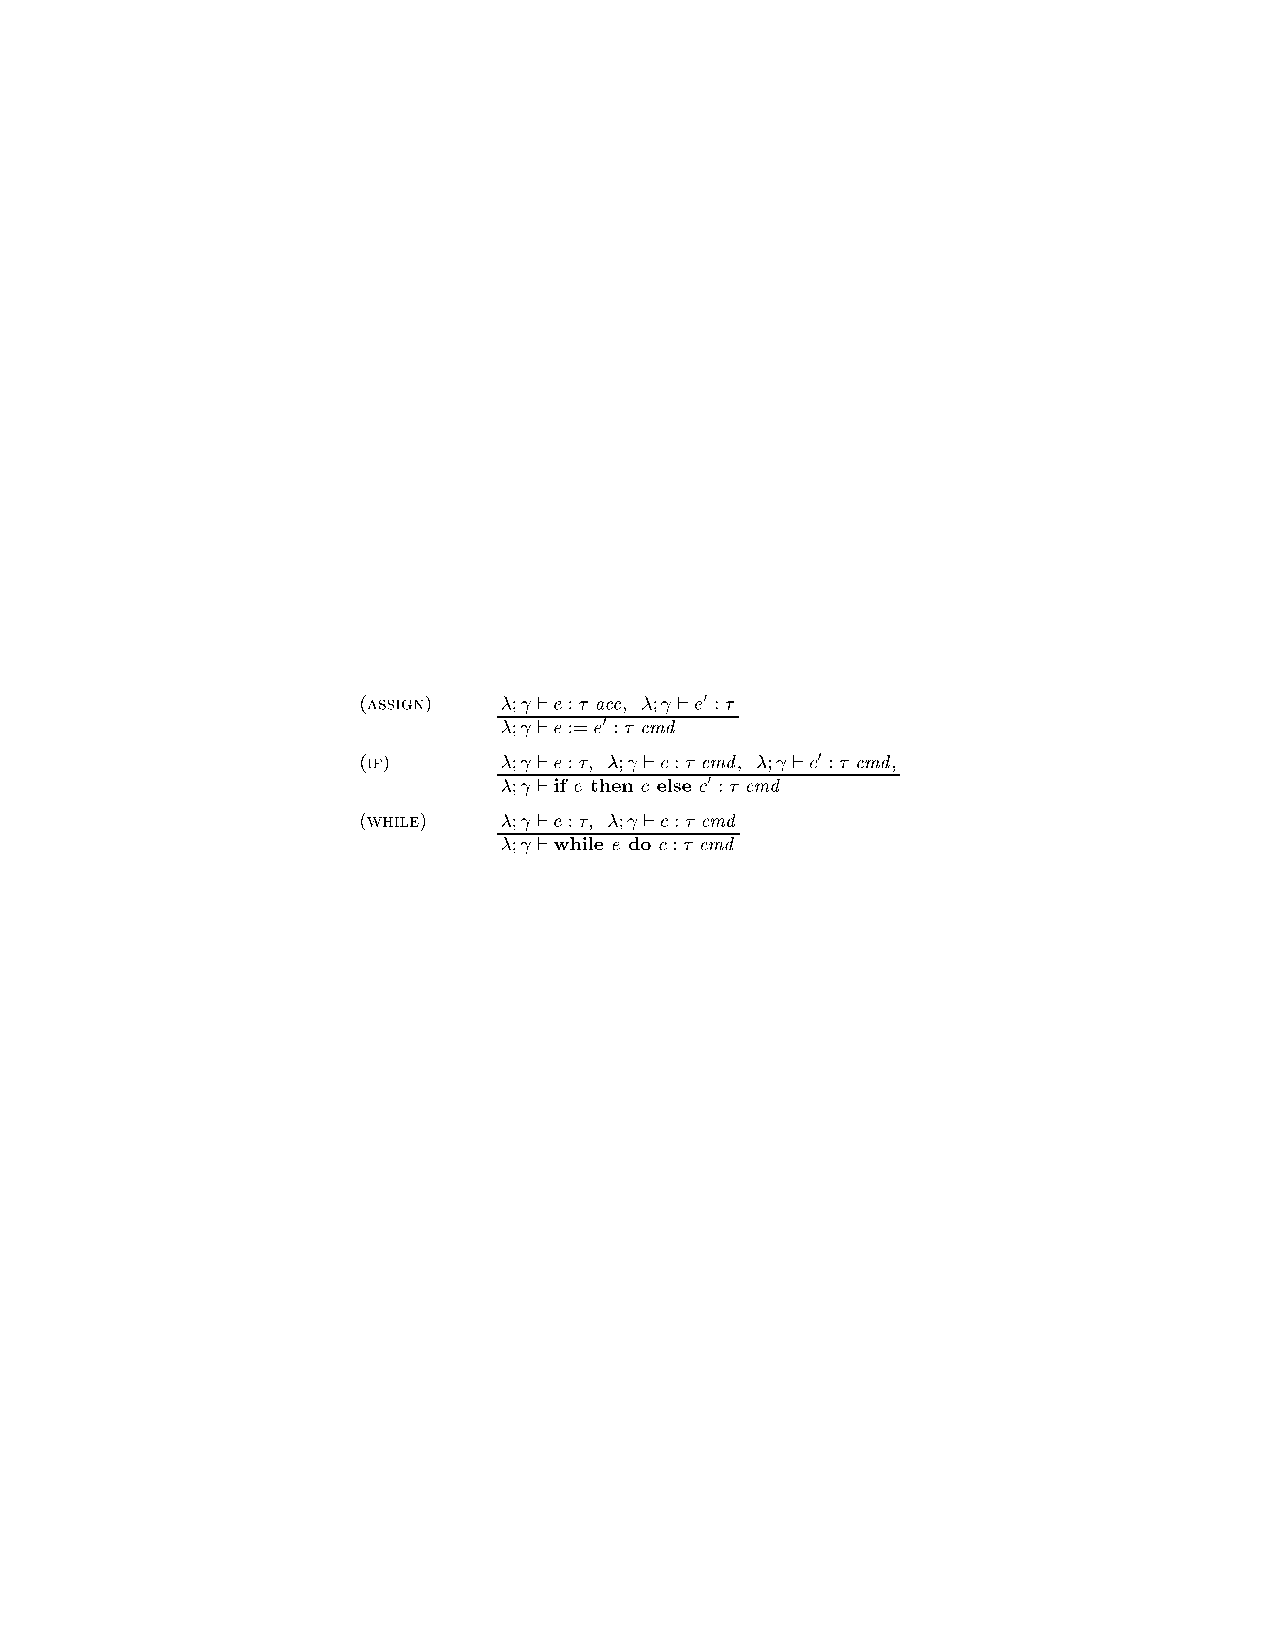
\includegraphics[scale=1.2]{figures/typesys3}
\end{center}
\end{frame}

\begin{frame}
\frametitle{Next time}
\begin{itemize}
\item Natural semantics for language
\item Noninterference as Type soundness argument:
\begin{itemize}
\item Argue that well-typed programs do not interfere.
\end{itemize}
\end{itemize}
\end{frame}

\end{document}
    











